\documentclass[12pt, a4paper]{article}

% -----------------------------
% Core Packages
% -----------------------------
\usepackage[margin=1in]{geometry}
\usepackage{graphicx}
\usepackage{xcolor}
\usepackage[colorlinks=true, linkcolor=blue!70!black, urlcolor=blue!70!black]{hyperref}
\usepackage{amsmath}
\usepackage{listings}
\usepackage{float}
\usepackage{helvet} % Modern sans-serif font for headings

% -----------------------------
% Graphics & Flowcharts (TikZ)
% -----------------------------
\usepackage{tikz}
\usetikzlibrary{shapes.geometric, arrows.meta, positioning, shadows}

\tikzstyle{workflowbox} = [
    rectangle, draw=blue!50!black, fill=blue!5, thick,
    text width=6cm, text centered, rounded corners=3pt,
    minimum height=3em, font=\sffamily\bfseries, drop shadow
]
\tikzstyle{arrow} = [thick, ->, >=stealth, draw=gray!80]

% -----------------------------
% UI Boxes (CompChems Style)
% -----------------------------
\usepackage[most]{tcolorbox}

% 1. Table of Contents Box
\newtcolorbox{tocbox}{
    colback=gray!5, colframe=gray!40,
    fonttitle=\bfseries\sffamily\Large, title=CONTENTS,
    coltitle=black, arc=4pt, boxrule=1pt,
    left=10pt, right=10pt, top=10pt, bottom=10pt
}

% 2. Syntax Breakdown Box (Blue)
\newtcolorbox{syntaxbox}{
    colback=cyan!5, colframe=cyan!60!black,
    fonttitle=\bfseries\sffamily, title=\faIcon{code} Syntax Breakdown, % Requires \usepackage{fontawesome5} if you want icons, omitted here for compatibility.
    title=Syntax Breakdown,
    arc=2pt, boxrule=1pt, left=8pt, right=8pt
}

% 3. Pro-Tip Box (Green)
\newtcolorbox{protip}{
    colback=green!5, colframe=green!50!black,
    fonttitle=\bfseries\sffamily, title=Pro-Tip,
    arc=2pt, boxrule=1pt, left=8pt, right=8pt
}

% 4. Warning/Gotcha Box (Orange)
\newtcolorbox{gotcha}{
    colback=orange!5, colframe=orange!70!black,
    fonttitle=\bfseries\sffamily, title=Watch Out!,
    arc=2pt, boxrule=1pt, left=8pt, right=8pt
}

% -----------------------------
% Code Block Styling
% -----------------------------
\lstset{
    language=bash,
    basicstyle=\ttfamily\small,
    keywordstyle=\color{blue!70!black}\bfseries,
    commentstyle=\color{green!50!black}\itshape,
    stringstyle=\color{red!70!black},
    numbers=left,
    numberstyle=\tiny\color{gray},
    stepnumber=1,
    backgroundcolor=\color{gray!5},
    frame=leftline,
    framerule=2pt,
    rulecolor=\color{blue!40},
    breaklines=true,
    captionpos=t,
    xleftmargin=15pt
}

% -----------------------------
% Document Setup
% -----------------------------
\title{\sffamily\Huge\bfseries Mastering Umbrella Sampling \\ \Large Mapping Cis--Trans Isomerization Free Energy}
\author{\sffamily Computational Chemistry Tutorials}
\date{}

\begin{document}

\maketitle

% -----------------------------
% Contents block
% -----------------------------
\begin{tocbox}
    \tableofcontents
\end{tocbox}
\vspace{2em}

% -----------------------------
\section*{About the tutorial}
\addcontentsline{toc}{section}{About the tutorial}
% -----------------------------
Standard molecular dynamics simulations often fail to capture rare events like cis--trans isomerization because the energy barrier is too high to cross at standard temperatures. The molecule will simply vibrate in its local energy minimum for microseconds.

To overcome this, \textbf{Umbrella Sampling (US)} applies an artificial biasing potential along a reaction coordinate (a dihedral angle, in this case) to force the simulation to sample high-energy transition states. By running multiple independent simulations across the entire dihedral space, we can mathematically remove the bias later using the \textbf{Weighted Histogram Analysis Method (WHAM)} to reveal the true Free Energy Surface (FES).

% -----------------------------
\section{Simulation Workflow}
% -----------------------------
The workflow requires us to physically force the transition to generate structures, and then run isolated production simulations for every step along that pathway.

\begin{figure}[H]
\centering
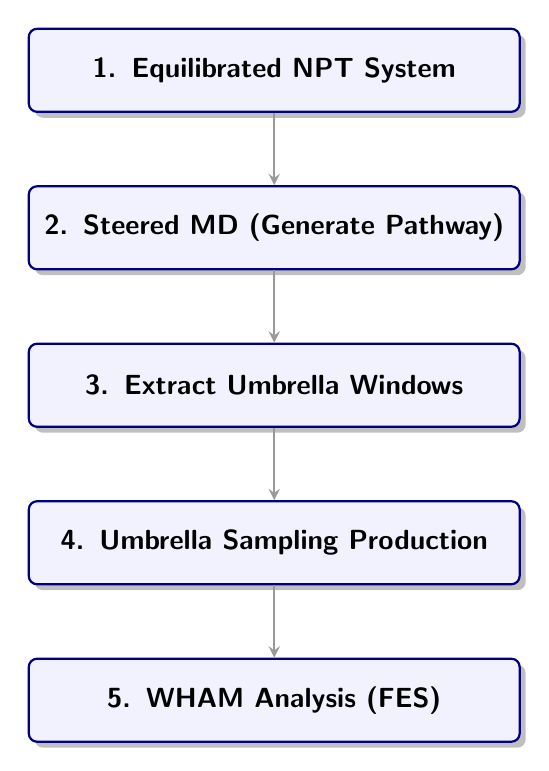
\begin{tikzpicture}[node distance=2cm]
    \node [workflowbox] (npt) {1. Equilibrated NPT System};
    \node [workflowbox, below of=npt] (smd) {2. Steered MD (Generate Pathway)};
    \node [workflowbox, below of=smd] (extract) {3. Extract Umbrella Windows};
    \node [workflowbox, below of=extract] (us) {4. Umbrella Sampling Production};
    \node [workflowbox, below of=us] (wham) {5. WHAM Analysis (FES)};
    
    \path [arrow] (npt) -- (smd);
    \path [arrow] (smd) -- (extract);
    \path [arrow] (extract) -- (us);
    \path [arrow] (us) -- (wham);
\end{tikzpicture}
\end{figure}

% -----------------------------
\section{Steered MD: Generating the Pathway}
% -----------------------------
We begin with an equilibrated \texttt{npt.gro} structure. To set up our umbrella windows, we need structures spanning the entire reaction coordinate ($-180^\circ$ to $+180^\circ$). We achieve this by "pulling" the dihedral angle using a moving harmonic restraint.

\subsection{PLUMED Steering Input}
Create a file named \texttt{plumed\_steer.dat}. 

\begin{lstlisting}[title={\textbf{plumed\_steer.dat}}]
# Define the dihedral angle
phi: TORSION ATOMS=6,12,13,18

# Apply a moving restraint from -pi to +pi
restraint: MOVINGRESTRAINT ARG=phi STEP0=0 AT0=-3.14 KAPPA0=1000 STEP1=500000 AT1=3.14 KAPPA1=1000

# Print the progress
PRINT STRIDE=100 ARG=phi,restraint.bias FILE=COLVAR
\end{lstlisting}

\begin{syntaxbox}
Let's break down the PLUMED parameters:
\begin{itemize}
    \item \texttt{phi: TORSION ATOMS=6,12,13,18} : Defines the coordinate using the atom indices that make up the rotatable bond.
    \item \texttt{MOVINGRESTRAINT} : Applies a time-dependent harmonic potential that changes its target over the course of the simulation.
    \item \texttt{STEP0 / STEP1} : The start and end integration steps of the pulling process.
    \item \texttt{AT0 / AT1} : The initial and final target angles.
    \item \texttt{KAPPA0 / KAPPA1} : The force constant ($kJ/mol/rad^2$) of the spring.
\end{itemize}
\end{syntaxbox}

\begin{gotcha}
\textbf{Radians vs. Degrees:} PLUMED uses radians by default. A common mistake is setting the \texttt{AT} target to \texttt{180} instead of \texttt{3.14} ($\pi$). PLUMED will attempt to pull your dihedral to 180 radians, which will instantly crash your simulation with a domain error.
\end{gotcha}

\subsection{Executing the Pull}
First, compile the binary input file, then pass the PLUMED file directly to \texttt{mdrun}.

\begin{lstlisting}[title={\textbf{Bash Execution}}]
gmx_mpi grompp -f steer.mdp -c npt.gro -p topol.top -n index.ndx -o steer.tpr 

mpirun -np 8 gmx_mpi mdrun -deffnm steer -plumed plumed_steer.dat
\end{lstlisting}

\begin{syntaxbox}
\begin{itemize}
    \item \texttt{-deffnm steer} : Sets "steer" as the default prefix for all output files (e.g., \texttt{steer.xtc}, \texttt{steer.log}).
    \item \texttt{-plumed plumed\_steer.dat} : Instructs GROMACS to link with the PLUMED plugin and apply the biases defined in the file.
\end{itemize}
\end{syntaxbox}

% -----------------------------
\section{Umbrella Sampling Production}
% -----------------------------
Assuming you have extracted the frames using a Python script (e.g., \texttt{extract\_windows.py}), you must now set up a separate directory for every window.

Unlike the moving restraint, Umbrella Sampling uses a \textbf{static} harmonic restraint centered exactly on that window's dihedral angle.

\begin{lstlisting}[title={\textbf{plumed.dat (Inside window\_05/ )}}]
phi: TORSION ATOMS=6,12,13,18
restraint: RESTRAINT ARG=phi AT=0.52 RAD KAPPA=2000
PRINT STRIDE=100 ARG=phi,restraint.bias FILE=COLVAR
\end{lstlisting}

\begin{syntaxbox}
\begin{itemize}
    \item \texttt{RESTRAINT} : Applies a static, unchanging harmonic bias.
    \item \texttt{AT=0.52} : The specific target center for this window. \textbf{This value must be updated for every single window folder.}
\end{itemize}
\end{syntaxbox}

\begin{protip}
The structures extracted from the pulling simulation are highly strained. It is strongly recommended to run a short (100 ps) NPT equilibration in each window with the static PLUMED restraint active \textit{before} starting your production run. This allows the solvent to relax around the artificially held solute.
\end{protip}

% -----------------------------
\section{WHAM Analysis}
% -----------------------------
Before generating the Free Energy Surface, check your \texttt{COLVAR} files to ensure the dihedral histograms for adjacent windows overlap. If they do not, your FES will have mathematical artifacts.

Once overlap is confirmed, concatenate the trajectories and use the PLUMED driver to evaluate the bias potentials.

\begin{lstlisting}[title={\textbf{Bash Execution}}]
gmx_mpi trjcat -cat -f umbrella_*/umbrella.xtc -o concatenated.xtc

plumed driver --mf_xtc concatenated.xtc --plumed plumed-wham.dat
\end{lstlisting}

\begin{syntaxbox}
\begin{itemize}
    \item \texttt{-cat} : Forces concatenation even if the times overlap.
    \item \texttt{--mf\_xtc} : Tells the PLUMED driver to evaluate a multi-frame trajectory.
\end{itemize}
\end{syntaxbox}

\end{document}